\documentclass{article}
\usepackage[T1]{fontenc}
\usepackage[utf8]{inputenc}
\usepackage[portuguese]{babel}

\usepackage{hyphenat}

\title{A preencher}
\author{Lucas Emanuel Resck Domingues}
\date{Novembro 2019}

\usepackage{natbib}
\usepackage{graphicx}
\usepackage{amsmath}

\begin{document}

    \maketitle

    \begin{abstract}
        A preencher
    \end{abstract}

    \section{Introdução}

    \section{Redes neurais \textit{feedforward}}

        Esta seção introduz uma configuração de redes neurais chamada \textit{feedforward}, como exemplifica a Figura \ref{fig1}, apresentada em \cite{nielsen2015neural}.

        \begin{figure}[h!]
            \centering
            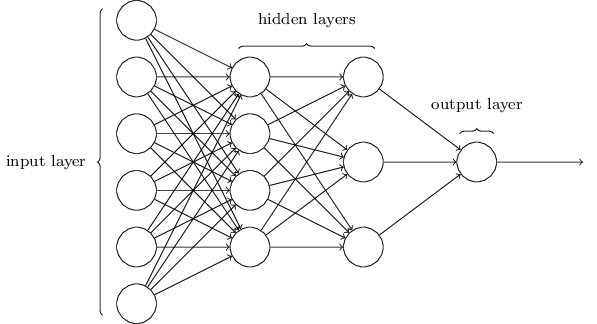
\includegraphics[scale=0.5]{Images/Feedforward neural network.png}
            \caption{Exemplo de rede neural \textit{feedforward}.}
            \label{fig1}
        \end{figure}        

        \subsection{Neurônios sigmóide}

            A unidade fundamental de uma rede neural é o neurônio, em analogia ao cérebro presente nos animais.
            Sejam $x_1, \cdots, x_n$ valores numéricos de entrada pertencentes a $[0, 1]$.
            Um neurônio é uma função que toma esses valores como entrada e produz uma saída, como exemplifica a Figura \ref{fig2}, também apresentada por \cite{nielsen2015neural}.

            \begin{figure}[h!]
                \centering
                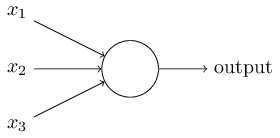
\includegraphics[scale=0.5]{Images/Sigmoid neuron.png}
                \caption{Exemplo de neurônio.}
                \label{fig2}
            \end{figure}
            
            Porém, esses neurônios não são uma função qualquer. Na verdade, podem ser descritos como:

            \begin{equation}
                \begin{split}
                    \textrm{output} &= \sigma(\mathbf{w} \cdot \mathbf{x} + \mathbf{b}) \\
                                    &= \dfrac{1}{1 + e^{-(\mathbf{w} \cdot \mathbf{x} + \mathbf{b})}}
                \end{split}
            \end{equation}

            $\sigma$ é a função sigmóide, daí o nome "neurônio sigmóide".

            $\mathbf{w}$ é um vetor de pesos, podendo ser interpretados como os pesos das arestas que ligam $x_i$ e o neurônio.
            Seu objetivo é "levar em consideração" \ todas as entradas, porém ponderando essas configurações.
            Veremos mais tarde, neste trabalho, que o objetivo da rede neural é "aprender" \ (também) quais os valores de $\mathbf{w}$.

            $\mathbf{x}$ é o vetor da entrada.
            
            $\mathbf{b}$ é um vetor de viéses.
            Quando os neurônios não usavam funções sigmóide, a saída era $0$ ou $1$.
            O objetivo do viés, então, era deslocar o parâmetro em que o neurônio seria "ativado" \ ou não.

            Observe que a saída do neurônio é uma função não linear de uma combinação linear das entradas.
            A combinação linear permite que ajustemos os pesos para a saída que quisermos, ou seja, "pequenas alterações na entrada produzem pequenas alterações na saída".
            A ideia é que não geramos saltos ou grandes variações quando alteramos apenas um pouco o parâmetro de entrada.
            
            O fato da função ser não linear é o que dá a complexidade da função quando muitos neurônios são reunidos.
            Veremos que, ao reunirmos vários neurônios para formar uma rede neural, teremos uma função não linear muito complexa.

        \subsection{Arquitetura}

            A arquitetura de uma rede neural tradicional se dá criando partições de um grafo.
            Observe novamente a Figura \ref{fig1}.
            A cada partição do grafo, chamaremos camada (\textit{layer}).
            Duas camadas "adjacentes" \ são totalmente conectadas, com todas as arestas orientadas no mesmo sentido (que, por convenção, será da esquerda para a direita).

            A primeira camada é chamada camada de entrada (\textit{input layer}).
            Tecnicamente, esta não é uma camada de verdade, mas apenas uma representação da entrada de valores, tal que os neurônios para os quais as arestas dessa camada apontam apenas recebem esses valores.
            
            A última camada é a de saída (\textit{output}).
            As camadas restantes são chamadas escondidas (\textit{hidden layers}), apenas por analogia.

            Vamos considerar a matriz $W_k$ sendo aquela com os pesos da camada $k$.
            Então o elemento $w_{ji}$ (linha $j$, coluna $i$) representa o peso da aresta que liga o nó $j$ da camada $k$ ao nó $i$ da camada $k + 1$.
            Além disso, $b_k$ representa os viéses de cada neurônio da camada $k$.
            
            Dessa forma, um vetor $\mathbf{x}$ na camada $k$ tem como resultado na camada $k + 1$ o vetor $\sigma (W_{ji} \mathbf{x} + \mathbf{b_k})$.
            Observe que a função $\sigma(\mathbf{x})$ aplicada ao vetor $\mathbf{x}$ representa a aplicação da função $\sigma$ a todos os elementos de $\mathbf{x}$.

            Sejam $W$ a matriz tridimensional de $W_k$ e $b$ a matriz de vetores $\mathbf{b_k}$.

        \subsection{Aprendizado com método do gradiente}
        
            Suponha que queiramos uma rede neural para diferenciar gatos e cachorros.
            Então construímos de forma que tenha dois neurônios na camada de saída.
            Queremos que, ao alimentarmos a rede com a imagem (vetorizada) e um cachorro, ela resulte em um vetor $(1, 0)$.
            Quando alimentada por uma imagem de um gato, $(0, 1)$.
            Buscamos um banco de dados de cachorros e gatos. Seja $\mathbf{y}$ a função que identifica cachorros e gatos:
            $$\mathbf{y}(\mathbf{x}) =  \begin{cases}
                                            (1, 0), & \textrm{se } \mathbf{x} \textrm{ representa um cachorro}, \\
                                            (0, 1), & \textrm{se } \mathbf{x} \textrm{ representa um gato}
                                        \end{cases}$$

            Se $a$ é a função que representa nossa rede neural e temos $n$ imagens, definimos a função \textbf{custo}: $$C(W, b) = \dfrac{1}{2n} \sum_{\mathbf{x}} ||\mathbf{y}(\mathbf{x}) - a(\mathbf{x}, W, b)||^2$$

            Nosso objetivo, nesse sentido, é calcular $W$ e $b$ tal que a função custo seja mínima.
            O método utilizado para isso é o do gradiente (\textit{gradient descent}), que atualiza os vetores $\mathbf{w_k}$ e $\mathbf{b_l}$ da seguinte forma:

            \begin{equation}
                \begin{split}
                    \mathbf{w_k} &\rightarrow \mathbf{w_k'} = \mathbf{w_k} - \eta \dfrac{\partial C}{\partial \mathbf{w_k}} \\
                    \mathbf{b_l} &\rightarrow \mathbf{b_l'} = \mathbf{b_l} - \eta \dfrac{\partial C}{\partial \mathbf{b_l}}
                \end{split}
            \end{equation}

            Porém, como o cálculo pode ser custoso, introduzimos o método do gradiente escocástico (\textit{stochastic gradient descent}), de modo que escolhemos uma amostra aleatória $X_1, \cdots, X_m$ do nosso banco de dados (um "mini-batch") e calculamos:

            \begin{equation}
                \begin{split}
                    \mathbf{w_k} &\rightarrow \mathbf{w_k'} = \mathbf{w_k} - \dfrac{\eta}{m} \sum_j \dfrac{\partial C_{X_j}}{\partial \mathbf{w_k}} \\
                    \mathbf{b_l} &\rightarrow \mathbf{b_l'} = \mathbf{b_l} - \dfrac{\eta}{m} \sum_j \dfrac{\partial C_{X_j}}{\partial \mathbf{b_l}}
                \end{split}
            \end{equation}

    \section{Rede de crença profunda}

        \subsection{Máquina de Boltzmann}

        \subsection{Máquina de Boltzmann restrita}

        \subsection{Rede de crença profunda}

    \section{Análise de redes neurais a partir de ciência de redes}

    \section{Considerações finais}

    \bibliographystyle{plain}
    \bibliography{references}
\end{document}
